%!TEX root = ../master.tex
\chapter{Testing and Evaluation}\label{ch:testeval}
In order to evaluate the product and see to what extent it can be considered successful, a usability test will be conducted.

\section{Purpose of test}
The purpose of this test is to test usability and functionality of the product. The ISO 9241 \citep{ISO} standard defines usability as effectiveness, efficiency, and satisfaction of the user. Put more precisely, this means:
\begin{itemize}
\item Efectiveness: To what extent are the goals of the product achieved?
\item Efficiency: What resources (including time) are expended to achieve the goals?
\item Satisfaction: To what extent does the user find the system acceptable?
\end{itemize}
With these in mind, the test aims to clarify whether the product lives up to its test objectives.

\section{Test objectives}
\todo{Andreas snakkede om at splitte objektiverne op i tech/usability, men spørgsmålet er om usability er det rigtige at bruge her eller om vi skal holde os til satisfaction}The problem statement is defined in Section~\ref{sec:ProblemStatement}. Based on this problem statement, it is important not only to test how well the program functions on a technical level, but also if the test participants still feel like they are playing the original board game, which will be tested on a level of satisfaction/acceptance.
The success criteria (Section~\ref{sec:SuccessCriteria}) and the system requirements (Section~\ref{sec:ReqSpec}) each add to the specifications on the technical and satisfaction  objectives of the test.

The technical oriented test objectives are:\todo{Capitalise every item and remove parentheses}
\begin{enumerate}
\setcounter{enumi}{0}
\item \begin{enumerate}
\item Does the player selection task live up to the requirement specification that it should be successful 90\% of the time? \label{req:1A}
\item Does the terraforming task live up to the requirement specification that it should be successful 90\% of the time? \label{req:1B}
\item The average delay time from the moment a gesture is done, to the moment the result can be seen on the interface should be around 3 seconds? \label{req:1C}
\item The average delay time from the moment a tile change is gestured, to the moment the result can be seen on the interface should be around 3 seconds? \label{req:1D}
\end{enumerate}
\end{enumerate}
The satisfaction oriented test objectives are:
\begin{enumerate}
\setcounter{enumi}{1}
\item \begin{enumerate}
\item Do the players still feel like they are playing Terra Mystica, when they are playing the augmented version? \label{req:2A}
\item Do the players feel like taking turns using the player selection gestures is an easy task, or a hindrance? \label{req:2B}
\item Do the players feel like the task of terraforming is easier to carry out than on the original board game? \label{req:2C}
\item Do the players feel that the augmented game board can replace the original game board? \label{req:2D}
\item How do the gestures for player selection and terraforming affect the pace of the game? \label{req:2E}
\end{enumerate}
\end{enumerate}

These objectives set the goals for the test, and help determine whether or not the test is successful. 

\section{Test methods}
To evaluate the product, two types tests are conducted. The first one is a technical tests using only group members, in order to test the technical aspects of the program, as this does not require participants from outside the group. The second type of test is the usability test, of which several will be conducted. These tests will focus on the satisfaction aspect of usability.

\subsection{Technical test}
\todo{technical test method goes here}
The purpose of the technical tests were to test the accuracy, effectiveness and overall efficiency of the system. The requirements for the tests were either completely adopted from or related to the test objectives. Specifically, requirements \ref{req:1A}, \ref{req:1B}, \ref{req:1C}, and \ref{req:1D} served as the aforementioned requirement inspiration.

The following requirements were formulated for the technical tests:
\begin{enumerate}
	\item \begin{enumerate}
		\item Effectiveness of each tile press (related to requirement 			\ref{req:1B})
			\begin{enumerate}
				\item This was tested by pressing each of the 112 hexagons on the board by hand, and if hand would fail, then with a hexagonically shaped paper template.
			\end{enumerate}
		\item Efficiency of colour change (related to requirement \ref{req:1D})
		\begin{enumerate}
				\item This was tested by timing the moment of table contact to the tile colour change in seconds.
		\end{enumerate}
		\item Hand or template used (related to requirement \ref{req:1B})
		\begin{enumerate}
				\item It was registered whether or not hand gesture would work for changing tiles. The output was used for generating a map of successes and fails to see hard-to-detect areas. Figure \ref{Fig:heatmap} is an example of this.
		\end{enumerate}
	\end{enumerate}
	\item \begin{enumerate}
		\item Effectiveness of player change gesture (related to requirement \ref{req:1A})
		\begin{enumerate}
				\item This was tested by using paper cut-outs to test successful detection of the respective players.
		\end{enumerate}
		\item Efficiency of player change gesture (related to requirement \ref{req:1C})
		\begin{enumerate}
				\item The times for each player hand detection were logged.
		\end{enumerate}
	\end{enumerate}
	\item \begin{enumerate}
		\item Effectiveness for undo action (Unrelated to requirements)
		\item Efficiency for undo action (Unrelated to requirements)
	\end{enumerate}
	\item \begin{enumerate}
		\item Number of restarts of code during technical tests (Unrelated to requirements, this was included as a way to track how automatic the code could function during the tests.)
	\end{enumerate}
	\item \begin{enumerate}
		\item Accuracy for tile changes made by hand (related to \ref{req:1B})
		\begin{enumerate}
				\item This was done by pressing 5 tiles (4 corners and 1 centre tile by hand and see if it was successful.
		\end{enumerate}
	\end{enumerate}
\end{enumerate}

\subsection{Participants for usability tests}
The chosen test participants are 16 young adult students from the AAU and they are our typical users. They are within the target group, which is defined in Section~\ref{sec:TargetGroup}, meaning that they are experienced with board games. We do not base our test on all participants being familiar with Terra Mystica, and therefore based the test design on participants just being familiar with board games in general. 

\subsection{Usability test set-up}
\begin{figure}[!h]
	\centering
	\begin{subfigure}[b]{0.4\textwidth}
	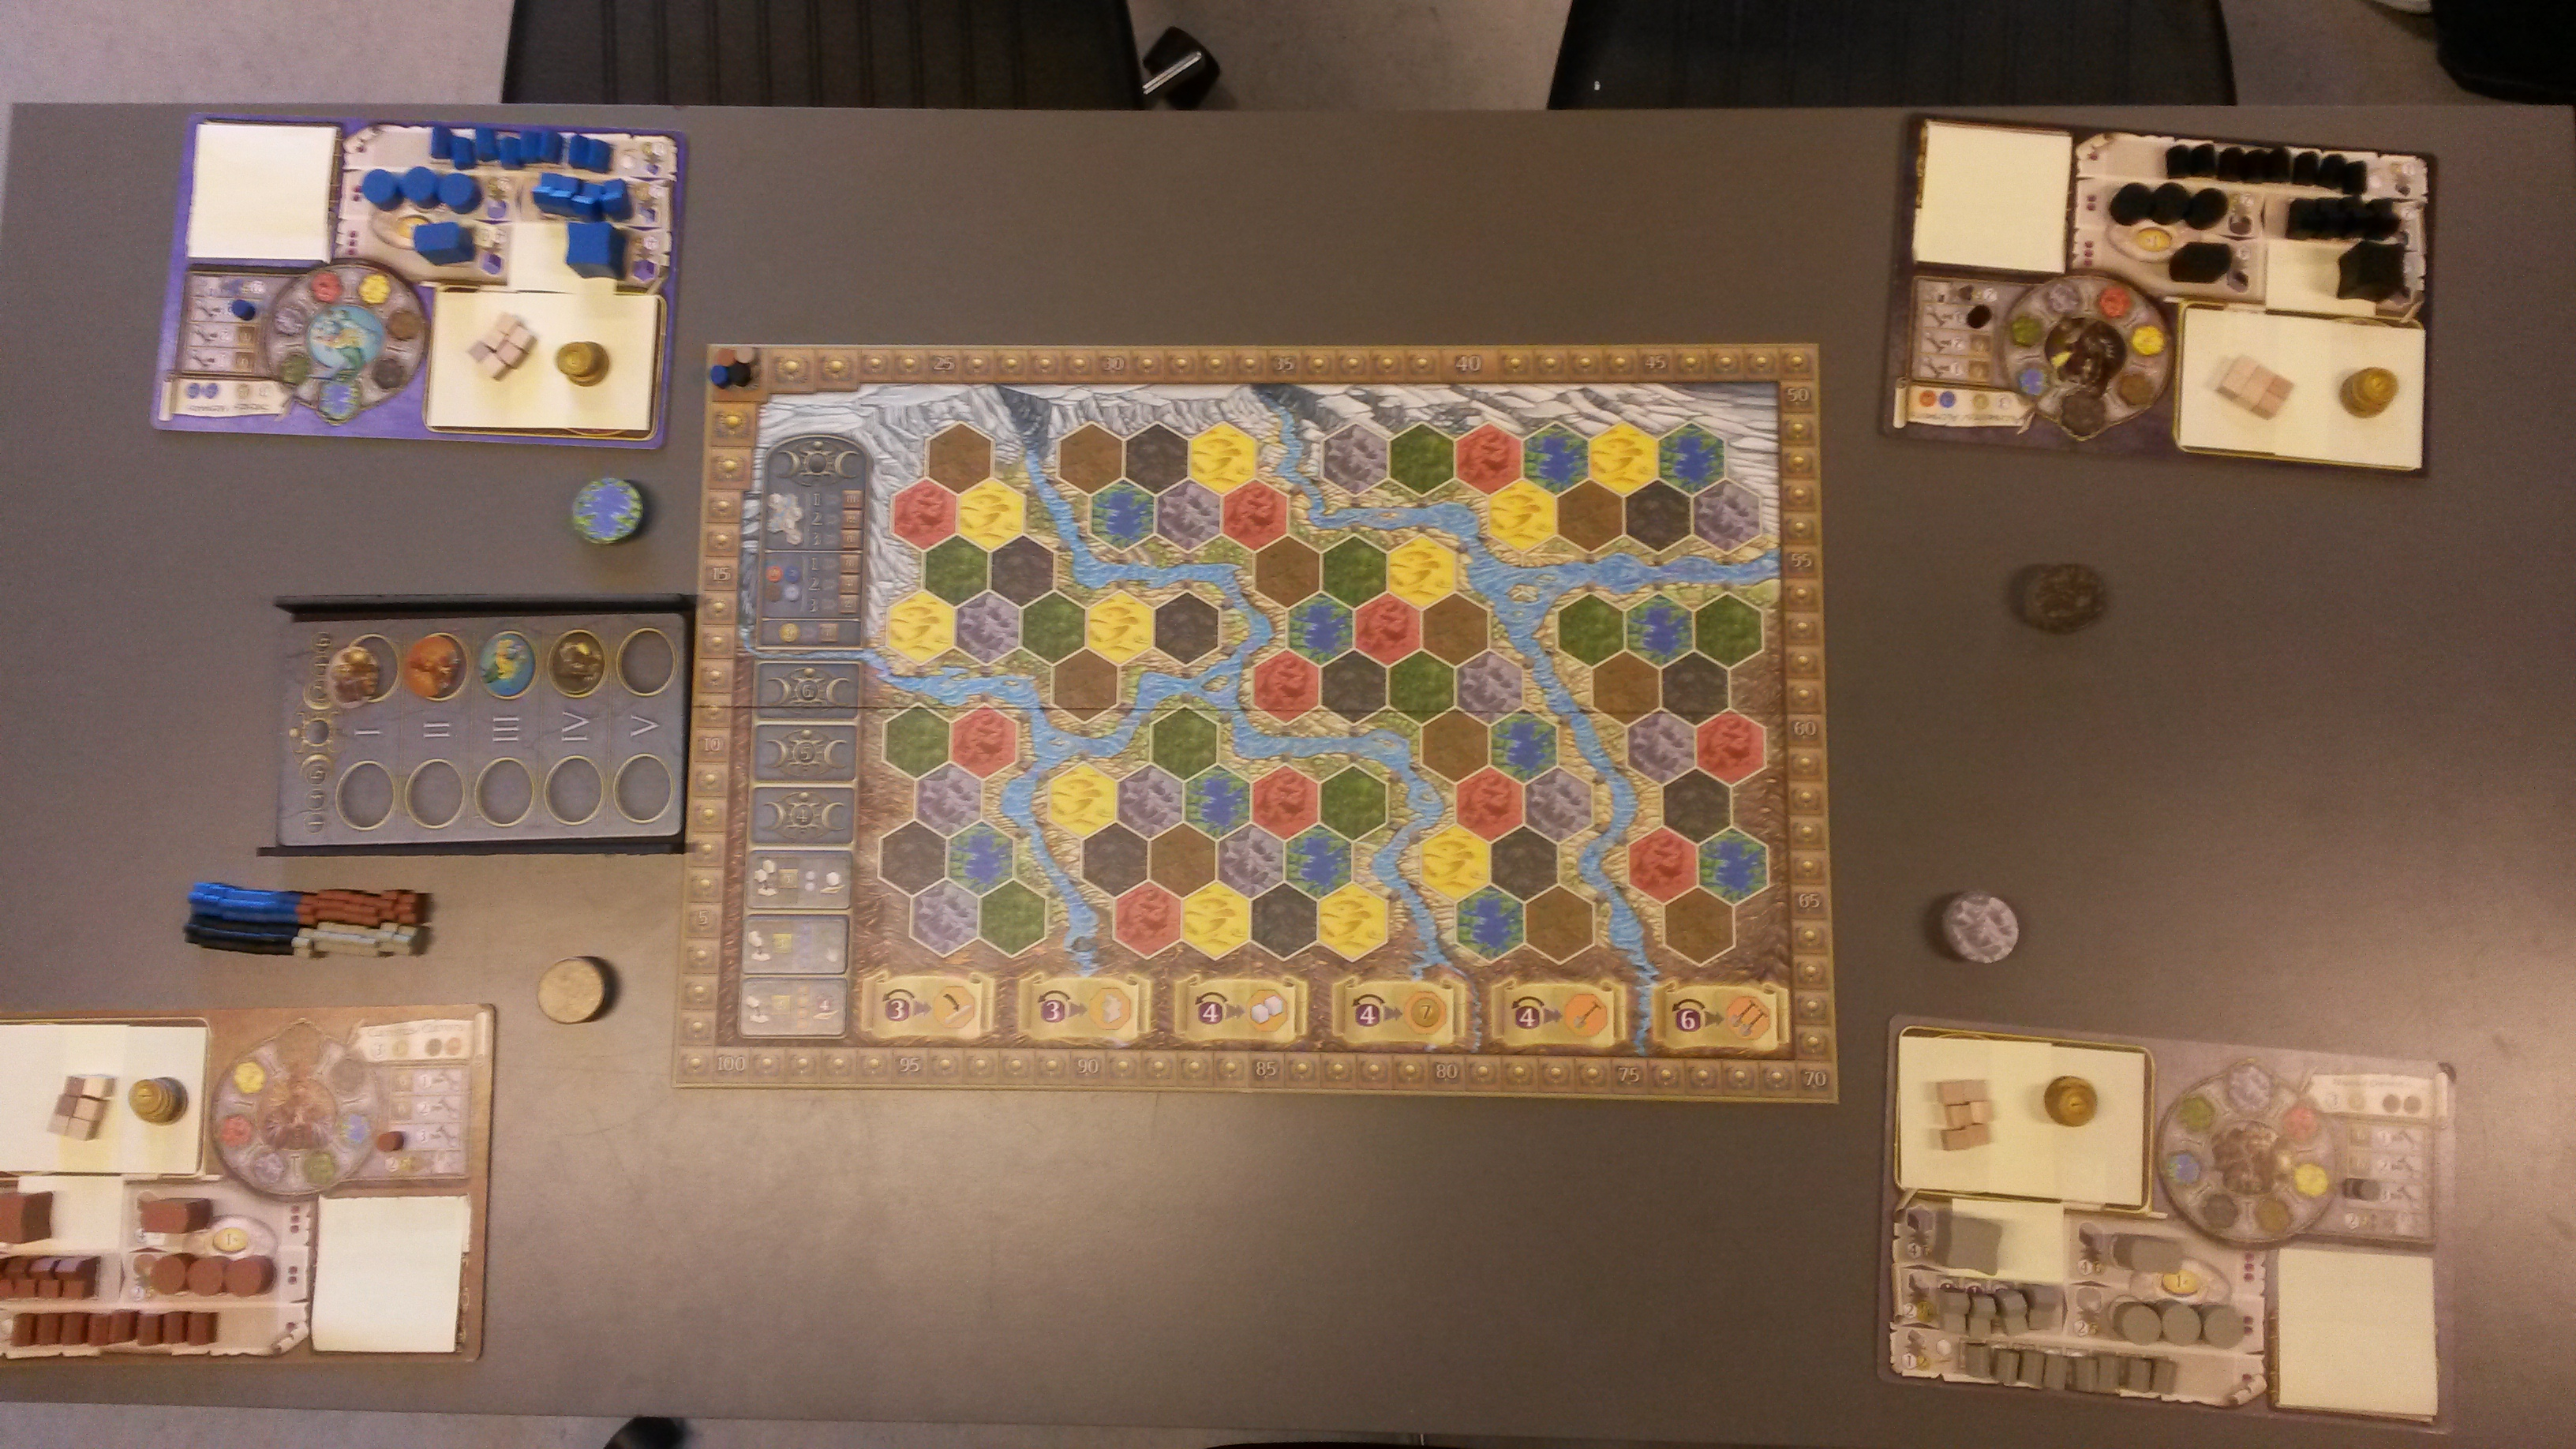
\includegraphics[width=\textwidth]{setup_analogue}
		\caption{\label{Fig:SetupAna}}
	\end{subfigure}
	\begin{subfigure}[b]{0.4\textwidth}
	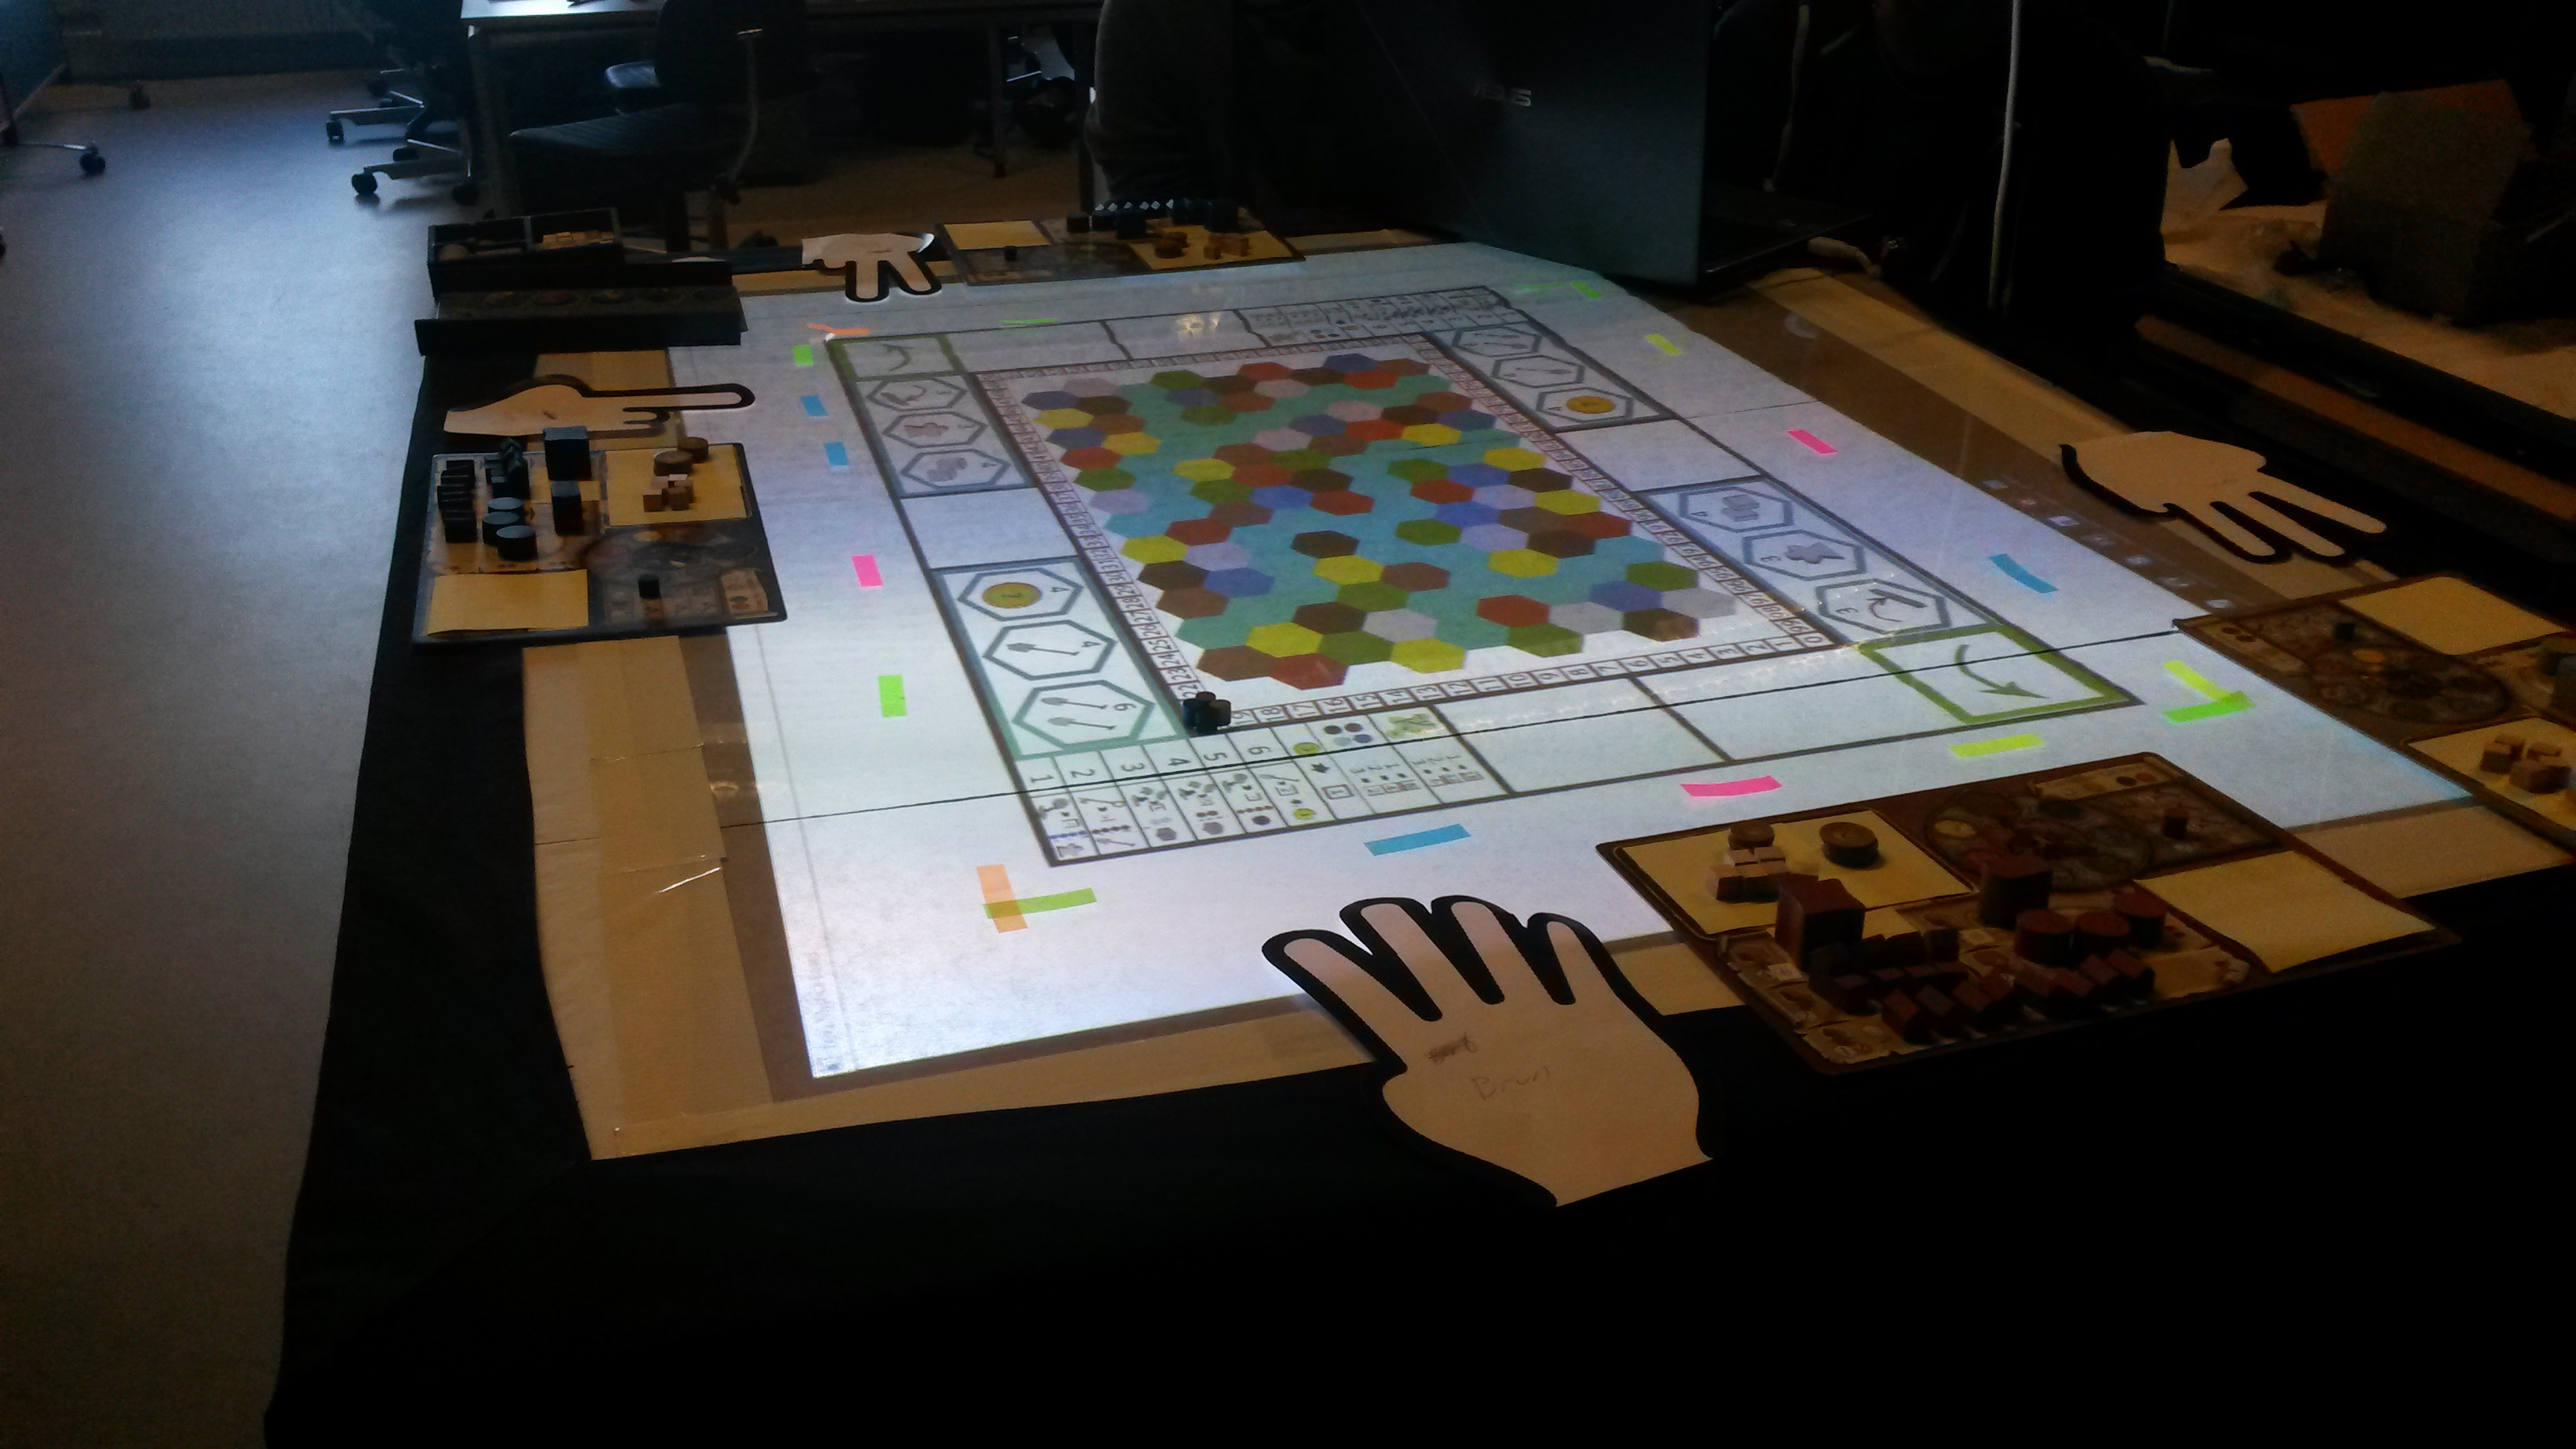
\includegraphics[width=\textwidth]{setup_digital}
		\caption{\label{Fig:SetupDigi}}
	\end{subfigure}
	\caption{Setup for the usability test, showing participants both the analogue game \textbf{(a)}, and the digital one \textbf{(b)}.\label{Fig:Setup}}
\end{figure}\todo{I don't know if we want these setup pictures or ones with participants on them. If we want the latter we can grab them from the video.}
The test takes place in the open study area, since the set-up requires a lot of room and the hardware will take up extra time to disassemble and reassemble, and moving it may dama the diffusor. Two tables are used for this test; one is the augmented board built for this project, and one is a table with the analogue game for comparison. The two setups can be seen in Figure \ref{Fig:Setup}. As the test includes people who are not experienced with Terra Mystica, several aspects of the game have been removed for simplicity's sake. These are covered up on each player's information board. Four test participants are placed around the table for each test, one by each information board, as well as four testers: One to operate a camera to record the test, one to take notes, one to explain the rules to the participants, and one to guide the participants and conduct the interview.

\subsection{Procedure for usability test}\todo{there will be changes here later on the week}
The test, when set up, will follow this procedure:

\begin{enumerate}
\item To begin with, the test guide will introduce the participants to the game and the project product, and then explain the whole test procedure. The guide will have a script to read from, which can be found in Appendix \ref{ch:TestScript}, to make sure all participants are fully informed.
\item Once all participants understand the procedure, they will play a game of Terra Mystica either using the augmented or original board for 3 rounds. After those 3 rounds are over, the participants will play a game with the board they have not tried yet. \todo{question is if we should add questions in between the games, since not only their comparison, but also initial impression might have significance} During the test introduction, they are encouraged to have dialogues with each other regarding their actions and thoughts as they play. This is inspired by the think aloud method addressed by Larsen \citep{TestingLecture}. The whole test is filmed by the cameraman. It is especially important to get footage of the participants' hands as they attempt to do gestures and as the related actions in the original version. It is likely that all of the typical tasks will be performed during this playthrough, but if not, the test guide will ask the test participants to attempt the ones they forewent.
\item Once the practical part of the test is over, the test guide will conduct a semi-structured group interview, which the participants have been informed about during the introduction. The participants will be asked about how they experienced the augmented game, both in its own right, and in comparison to the original game.
\end{enumerate}

Once the test is done, the footage and notes from the test will be analysed and compared to the test objectives.

\section{Results}
\subsection{Technical}
\subsection{Satisfaction}
All the four participant groups felt they were still playing Terra Mystica in both versions of the game. This was definitely due to the game mechanics still being the same in both versions, and to a less extent was it due to them saying that they ‘felt’ it was the same game. However, one group of participants stated that the digital version provided the same sense of ‘togetherness’ as the original version. In one group, it was mentioned that playing the augmented and the original versions each had their unique flair, and added something more to the game, with the examples of the digital version being dramatic/exciting and the original being comfortable/casual. 

All groups found the turn taking complicated in the digital version. One reason for this is that they had to place a paper hand in the middle of the board, which conflicted with already placed game pieces that it could accidentally displace. Additionally, some players forgot to switch turns on the digital board, as well as how they were supposed to do it, which they also stated as a problem with the design. Throughout the groups, a wish for some feedback regarding turn switching was expressed. It was suggested to either display the colour of the currently selected player, or to highlight their player area, in order to emphasize whose turn it is at the moment. On that matter, some participants also asked for a digital overview of the turn order, possibly with one close to each player’s area, so everyone has an easily available overview. 

While nobody directly said the task of terraforming was not easier to carry out in the augmented version, it was mentioned that the technical difficulties made the task take a long time, slowing down the augmented game. Several participants provided suggestions for improvements or alternatives to the terraforming feature. Examples of these suggestions are:
\begin{itemize}
\item An undo/reset-button for misplaced terraformings. Pressing this button would revert the latest action taken.
\item Multiple-choice terraforming instead of terraforming based on turn selection
\item A tool specifically for terraforming instead of using fingers, which mostly was advised, due to the participants experiencing the template hex taking over terraforming when the fingers did not suffice. An important note here is that in one of the groups all the participants saw the tool use as redundant, since they saw a tool for terraforming equal to using game pieces.
\end{itemize}
Besides that, participants mentioned that they expected the terraforming to be quite easy, if the system worked properly. 

The participants had very mixed opinions on which version they would prefer to play, and whether the augmented game board can replace the original one.

One participant stated that they would prefer not a mixture of digital and tactile elements, but a complete digital replacement of the board game, without any game pieces, since they found them frustrating. However, many enjoyed the tactile elements of the augmented game. While no test participants thought the augmented version can replace the original game in its current state, several participants showed interest in the augmented design, and thought it can potentially replace the original game, assuming that all mechanics will be properly implemented, and the major technical problems are removed. The augmented version would also need to have less similar colours in order to replace the original, according to several participants.

One participant, who was already experienced with Terra Mystica, noted that because of the augmented version’s simplistic design, they saw potential in it introducing new players to the game. It was also mentioned that the simplistic design provides a clearer overview over the map for players who are not famillar with the different terrain types. One participant noted that some of the elements of the game are insufficiently explained in the original version, and that the augmented version could compensate for that by having clearer explanations on its interface.

Some participants stated that the digital version of the game provided a different atmosphere, and mentioned that the augmented and original version game each served their purposes, implying that the augmented version would replace the original one in the right circumstances. To describe the augmented version, some participants used the words ‘dramatic’ and ‘intense’, stating that they felt they had more influence in the game, due to the direct interaction with the board’s surface.

All the groups felt that the original version of Terra Mystica went faster than the augmented version, due to the technical delays and difficulties. These groups also mentioned that they would expect the final version of the augmented version to be as fast - if not faster, than the original version. The reasons why it would be faster, as mentioned by participants, is all the points and currency management the augmented version could take care of. This could mean the current gestures for player selection and terraforming do affect the pace of the game negatively, slowing it down, but when improved, it might not affect the game pace differently than in the original version.

\subsection{Analysis}
text\todo{analysis and conclusion}